\documentclass{sig-alternate-05-2015}
\usepackage{graphicx}
\graphicspath{ {images/} }
\begin{document}

% Copyright
\setcopyright{acmcopyright}

\title{Modelling Relationships in Autonomous Systems and inter-domain Routing policies}

\numberofauthors{3} %  in this sample file, there are a *total*
% of EIGHT authors. SIX appear on the 'first-page' (for formatting
% reasons) and the remaining two appear in the \additionalauthors section.
%
\author{
% You can go ahead and credit any number of authors here,
% e.g. one 'row of three' or two rows (consisting of one row of three
% and a second row of one, two or three).
%
% The command \alignauthor (no curly braces needed) should
% precede each author name, affiliation/snail-mail address and
% e-mail address. Additionally, tag each line of
% affiliation/address with \affaddr, and tag the
% e-mail address with \email.
%
% 1st. author
\alignauthor Abhinav Agshikar\\
       \email{abhinav.agshikar}
% 2nd. author
\alignauthor
Sagar Thakkar\\
       \email{sagar.thakkar}
% 3rd. author
\alignauthor
Arnav Gupta\\
       \email{arnav.gupta}
}


\maketitle
\section*{PROBLEM STATEMENT}
Internet Measurement - modeling relationships in Autonomous Systems (ASes) and Inter-domain routing policies using CAIDA dataset and RIPE Atlas. 

\begin{abstract}
In this two part project, we plan to understand the relationships between Autonomous Systems (ASes) on the Internet and derive inferences
between theoretical and practical routing scenarios. For the first part of the project, we use the March 2016 CAIDA Dataset  [3] that 
represents a theoretical model of the AS relationships using the now standard Gao-Rexford model  [1] and create
a graph visualization using Neo4j [4] graph database. We present our analysis using statistics obtained with this dataset and pick the top 100
mostly connected ASes and use them for further analysis. In the second part  of the project that we will progress next,
we will explore practical routing scenarios using RIPE Atlas framework by using probe nodes found in the first part and find out routing
instabilities at inter-AS routing level.

\end{abstract}

\keywords{Autonomous Systems; Gao-Rexford Model; RIPE Atlas; BGP; Graph Database}

\section{Introduction}
\subsection{BGP and Autonomous Systems}
In the Internet, different ISPs communicate with each-other. These ISPs communicate with their customers using various Intra-domain routing protocols whose decision is made by the provider itself. They can decide the protocol based on their network traffic and distribution of customers in the geographical area (topology). However all these ISPs have to communicate with each other via a common protocol. This protocol which is agreed by the entire Internet community is called Border Gateway Protocol (BGP). The interdomain (exterior) routing paradigm is driven by the BGP communication between the Autonomous Systems (ASes). These Autonomous Systems are the exit point of a particular network driven by a network provider. These ASes communicate with other ASes based on certain policies. These policies are varied and is explained by now standard and accepted Gao - Rexford model.

\subsection{Gao - Rexford Model\textsuperscript{[1]}}
Generally while running a protocol to setup routes to the destination, it is typically done in a dynamic fashion via path vector-based implementation. However this protocol complexity lies in the set of routing policies each AS implements. To converge to a particular destination, there are often different ASes to traverse. A standard approach may be selecting the shortest path or the least cost path. However this is not true in all the cases, in practice the selection of ASes is based on various other factors including but not limited to financial policies between ISPs and amount of traffic to traverse the network. Due to this, there are always anomalies in the shortest path and the selected path in practical scenarios. Gao - Rexford model provides a set of guidelines that an AS can implement to set up its routing policies without coordination with other ASes and guarantee the convergence of path. This model gives us the ideal path between the ASes. We then compare the actual path and find anomalies in BGP routing in this project. We obtain the ideal connection details between ASes from CAIDA data set and the Actual connection using RIPE Atlas.

\subsection{CAIDA Dataset\textsuperscript{[4]}}
CAIDA stands for Center for Applied Internet Data Analysis. CAIDA curates datasets resulting from both active and passive Internet measurement and has been used
in several research papers. The dataset establishes relationships using the Gao-Rexford model. We use this information provided by CAIDA and obtain a list of ASes that are critical to the Internet infrastructure. Later we work to obtain the AS Topology map using this dataset.

\subsection{RIPE Atlas\textsuperscript{[5]}}
RIPE Atlas is a global, open, distributed Internet measurement platform, consisting of thousands of measurement devices that measure Internet connectivity in real time. Each AS has a probe sitting at the node to measure the network information. All these devices contribute to the Atlas community to share the information. We then use this information of ping and traceroute to identify the anomalies.
The RIPE Atlas has a number of restrictions with respect to the measurements that can be done-
\begin{enumerate}
\item No more than 100 simultaneous measurements for a single user
\item No more than 500 probes may be used per measurement
\item No more than 10 traceroute or ping UDMs can exist for a given target URL/IP for all users of the system. The condition does not apply to DNS measurements

\end{enumerate}
We plan to choose a set of Vantage points by picking up interesting ASes from list obtained from CAIDA.

\section{Problem Description}
The Internet has quickly evolved into a vast global network owned and operated by thousands of different administrative entities. During this time, it became apparent that vanilla shortest-path routing would be insufficient to handle the myriad operational, economic, and political factors involved in routing. ISPs began to modify routing configurations to support routing policies, i.e. goals held by the router's owner that controlled which routes were chosen and which routes were propagated to neighbors. When BGP was first introduced, it was a fairly simple path-vector protocol. Over time, many incremental modifications to allow ISPs to control routing were proposed and added to BGP. The end result was a protocol weighted down with a huge number of mechanisms that can overlap and conflict in various unpredictable ways. These modifications can be highly mysterious since many of them, including the decision process used to select routes, are not part of the protocol specification. Moreover, their complexity gives rise to several key problems, including unforeseen security vulnerabilities, widespread misconfiguration, and conflicts between policies at different ISPs.


The main task of the autonomous systems is to exchange network reachability information with other ASes.  This network reachability information includes information on the list of  Autonomous Systems that reachability information traverses. This information is sufficient for constructing a graph of AS connectivity for this reachability from which routing loops may be pruned, and, at the AS level, some policy decisions may be enforced. Models of Internet routing are critical for studies of Internet security, reliability and evolution, which often rely on simulations of the Internet's routing system. Accurate models are difficult to build and suffer from a dearth of ground truth data, as ISPs often treat their connectivity and routing policies as trade secrets. In this environment, researchers rely on a number of simplifying assumptions and models proposed over a decade ago, which are widely criticized for their inability to capture routing policies employed in practice.

Routing anomalies are commonly seen on Internet in day-to-day life. They range from simple misconfigurations in the internal infrastructure of ISP to faulty BGP updates in the Internet's control-plane that seriously affect the connectivity of entire countries or geographic regions. Amongst the various routing anomalies that exist, the project strives to examine a subset of them that connect to major causes of traffic filtering, misdirection and interception. Depending on the type of routing anomaly and whether it is occurring in the Internet's control- or data-plane, a number of different approaches can be taken to detect it. Anomalies are examined by a collection of steps that employ various datasets so that concise detection can be achieved. Hence given the vast size of the Internet it is of utmost importance to have a carefully chosen set of points through which to sense for such anomalies.


Analyzing and modelling the Internet topology is of immediate practical interest, since knowledge of the network's topological properties enables researchers to optimize network applications and to conduct more representative network simulations. The first reason might be to reduce bandwidth costs by preferring particular paths. The other is for performance reasons, where a particular transit provider may have less-congested/lower-latency path to a destination network. Network operators will view a variety of metrics to determine if there is a problem and start to make policy changes to examine the outcome. The links between various networks on the Internet today operate where they scale capacity based upon observed utilization. Even one may be paying a transit provider for connectivity, this doesn't mean every link to external networks is scaled for the amount of traffic. As traffic grows, links will be added between individual networks. So causing a massive change in utilization on the Internet can result in congestion as these new paths are handling an increased amount of traffic than they never had before. 

In order to determine the paths traffic is taking, tools known as traceroute is very useful. Traceroute operates by sending sending packets to a given destination network and it sets the initial IP TTL value to one. The RIPE Atlas provides a framework to provide results for. Thus the problem area which motivates us is to ensure the authenticity and consistency of practical routing information versus theoretical model governed by Gao Rexford. To do this we have appropriately taken two frameworks - CAIDA dataset (Theoretical model) and RIPE Atlas (Practical model) and perform analysis on these in real world scenarios.

\section{Solution Methodology}

We decided to split our project into two parts: AS Structure Visualization and AS BGP practical routing. For part 1, we used the CAIDA dataset to obtain AS relationships existing as of March 2016. We obtained two files - AS Rel file that contains AS-AS relationship mapping which can either be Peer to Peer or Provider to Customer. The other file contained a list of existing connections between ASes from where we identified most prominent ASes that has maximum connections. We retrieved a list of 100 most connected list of ASes and found their corresponding relationships in the first file. This gave us a list of 28846 unique ASes that we visualized using Neo4j.
For remaining portion of the project, we will work on RIPE Atlas traceroutes.

\section{Evaluation and Results}
\subsection{Analysis on CAIDA Dataset}
We first performed analysis on entire CAIDA dataset as of March 2016. The summary of this set is listed below:

\begin{center}
\begin{tabular}{ |c|c|c| } 
 \hline
 No of Unique ASes & 53537 \\ 
 \hline
 No of Links & 406401 \\ 
 \hline
\end{tabular}
\\Table 1: Statistics of Complete Dataset\\
\end{center}

We next narrowed this dataset by using the top 100 most connected ASes. We list summary and top 5 most connected Ases these below:

\begin{center}
\begin{tabular}{ |c|c|c| } 
 \hline
 No of Unique ASes & 28846 \\ 
 \hline
 No of Links & 68712 \\ 
 \hline
\end{tabular}
\\Table 2: Statistics of Reduced Dataset\\
\end{center}



\begin{center}
\begin{tabular}{ |c|c|c| } 
 \hline
ASN &  Name & Country \\
 \hline
ASN3356 &  Level 3 Communications, Inc. & USA \\
 \hline
ASN174 & Cogent Communications & USA \\
\hline
ASN1299 & TeliaSonera AB & Europe \\
\hline
ASN2914 & NTT America, Inc. & USA \\
\hline
ASN3257 & Tinet Spa & HongKong \\
\hline
\end{tabular}
\\Table 3: Top 5 most connected ASes\\
\end{center}
\begin{center}
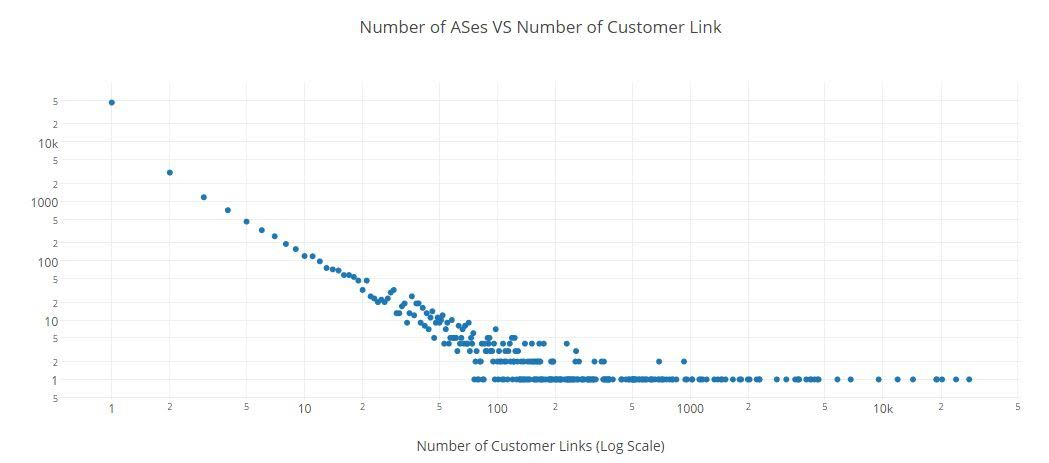
\includegraphics[scale=0.2]{graph1}\\
Fig 1. Scatter Plot of AS vs Number of links\\
\end{center}
The scatter plot above indicates that there are very few nodes having huge number of links (Peer-Peer and Provider-Customer). Around 15000 ASes have only one link while the highest number of links were around 28000.
\subsection{AS Relationship Visualization and Inferences}
Now we used Neo4j which is a graph database for visualizing these ASes. We created two CSVs containing the two relationships i.e.
Provider to Customer and Peer to Peer. We initially created the total list of 28846 nodes in the database and then input the relationships files.
\begin{center}
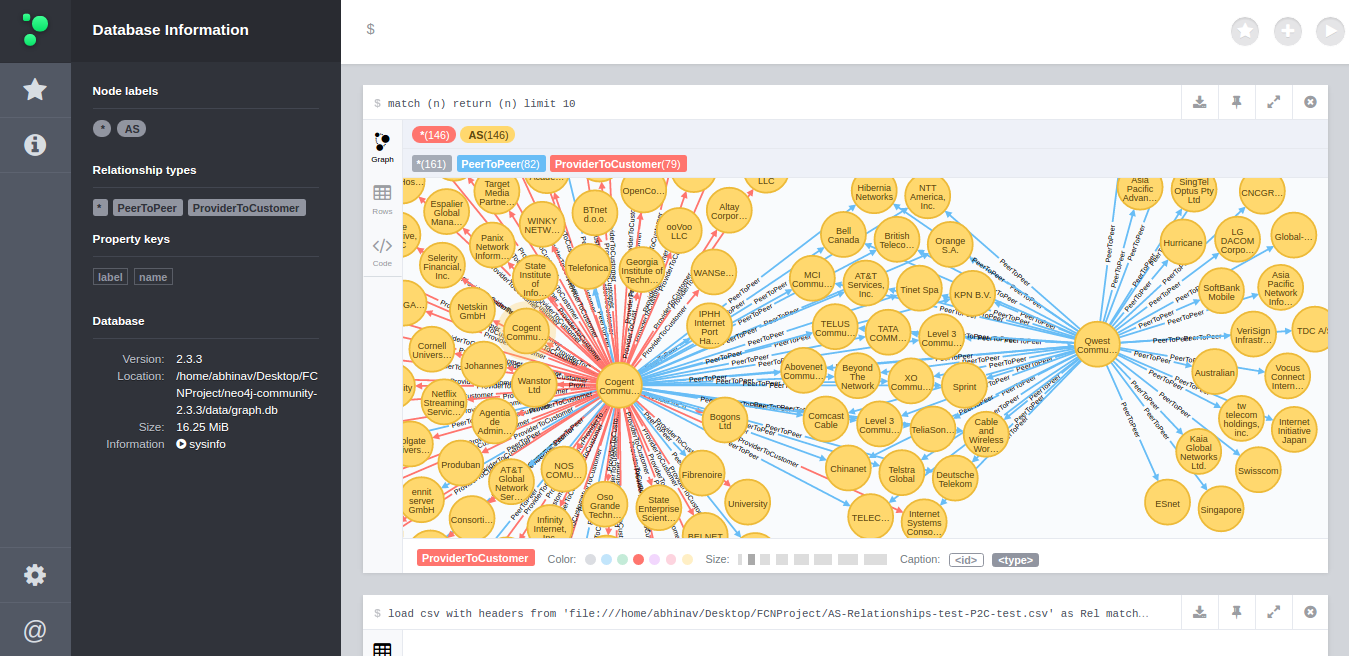
\includegraphics[scale=0.18]{graph2}\\
Fig 2. Visualization of Cogent and Qwest Communication ASes\\
\end{center}

\begin{center}
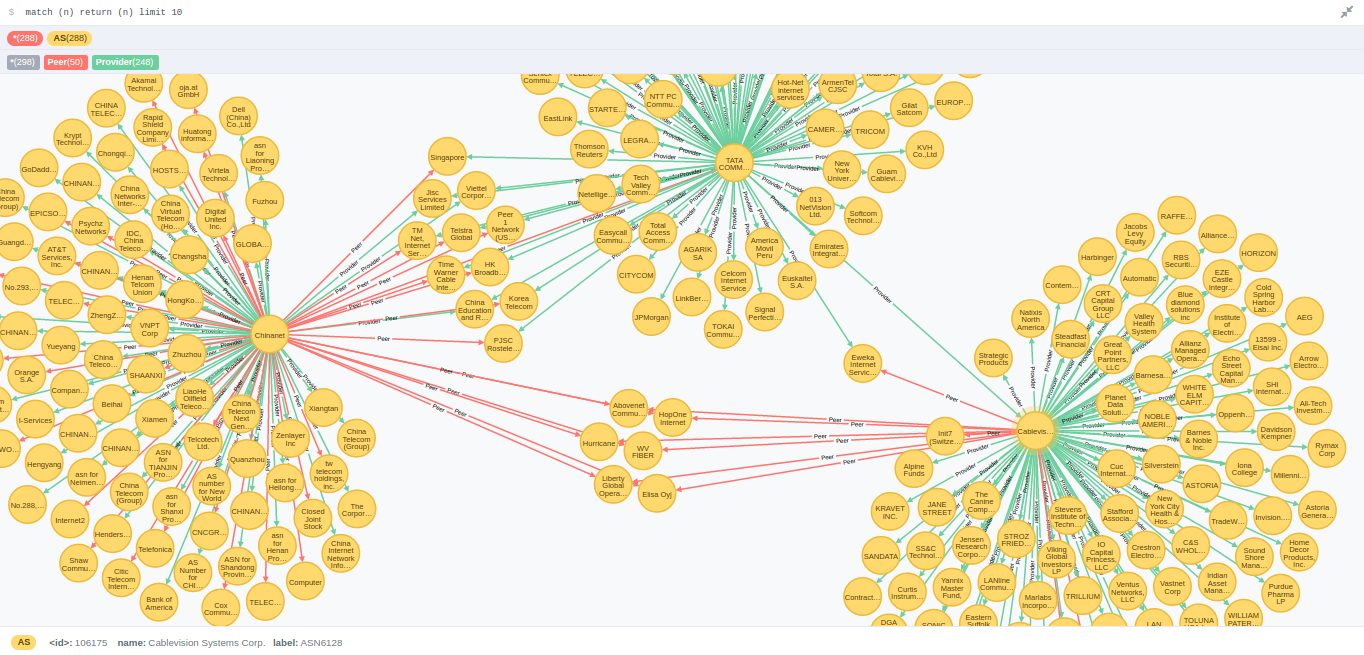
\includegraphics[scale=0.18]{graph3}\\
Fig 3. Visualization of ChinaNet vs Cablevision vs Tata Comm (US) \\
\end{center}
One of the interesting results that we could see is that the more highly linked ASes have 
very few Peer-Peer relationships with other ASes compared to a larger portion of Provider-Customer relationships.

\subsection{RIPE Atlas}
Amongst the top 100 highly connected list of ASes, we identified three particularly interesting ones that can be helpful in our further
analysis with RIPE Atlas -
AS6128: Cablevision Systems, AS6453: Tata Comm (US), AS4134: ChinaNet. For these three ASes, we found existing Internet Measurement
probes as follows:
\begin{center}
\begin{tabular}{ |c|c|c| } 
\hline
ASN &  Name & Atlas Probe IDs \\
 \hline
AS6453 &  Tata Comm (US) INC & 19797 \\
 \hline
AS6128 &  Cablevision Systems Corp. & 23478,22723, .. \\
 \hline
AS4134 &  ChinaNet & 23846,15504, .. \\
 \hline
 \end{tabular}
 \\Table 4: Vantage Points\\
\end{center}

\section{Future Work}
For the next part of our project, we will continue working on ATLAS RIPE. We have the connectivity information of the ASes which we will compare with the traceroute and ping responses dump available on the RIPE Atlas website for the Probe IDs corresponding to those ASes.
\begin{enumerate}
\item Use RIPE ATLAS ping and traceroute dump for the identifying the anomalies in the inter AS routing. This we plan to do by comparing the connectivity details we obtained for different vantage points in part 1 of the project. 
\item The anomalies which we plan to work upon includes but not limited to Identifying the bogus prefixes in the traceroute and mismatch between the Gao - Rexford model solution provided by the CAIDA dataset and the measurement information we obtained from the ATLAS dataset.


\end{enumerate}

\section{Acknowledgements}
We would like to thank Professor Aruna for her involvement in constant discussions through the progress of this project. We would also like to thank Professor Phillipa for her feedback on Internet Measurement and possible applications areas for RIPE Atlas.

\section{References}
1. ``Stable Internet Routing without Global co-ordination" - Lixin Gao, Jennifer Rexford\\
2. ``Investigating Interdomain Routing Policies in the Wild'' - Ruwaifa Anwar, Haseeb Niaz, et al\\
3. CAIDA datasets - http://data.caida.org/datasets \\
4. Neo4j Graph Database - http://neo4j.com\\
5. RIPE Atlas https://atlas.ripe.net\\
\end{document}
